\subsection{Experimental Setup}
\label{sec:setup}

\subsubsection{System used}

We use a server outfitted with two Intel Xeon Gold 6226R processors. Each processor comprises $16$ cores operating at $2.90$ GHz. Each core has a $1$ MB L1 cache, a $16$ MB L2 cache, and a shared L3 cache of $22$ MB. The system is set up with $376$ GB of system memory and has CentOS Stream 8 installed.


\subsubsection{Configuration}

We employ 32-bit integers to represent vertex IDs and 32-bit floats for score computation. We utilize $32$ threads to match the system core count (unless specified otherwise). Compilation is carried out using GCC 8.5 and OpenMP 4.5.


\subsubsection{Dataset}

The graphs used in our experiments are given in Table \ref{tab:dataset}. These are sourced from the SuiteSparse Matrix Collection \cite{suite19}. In the graphs,\ignore{the} number of vertices vary from $3.07$ to $214$ million, and\ignore{the} number of edges vary from $25.4$ million to $3.80$ billion. We ensure that edges are undirected and weighted with a default of $1$.

\begin{table}[hbtp]
  \centering
  \caption{List of $13$ graphs obtained SuiteSparse Matrix Collection \cite{suite19} (directed graphs are marked with $*$). Here, $|V|$ is the number of vertices, $|E|$ is the number of edges (after adding reverse edges), $D_{avg}$ is the average degree, and $|\Gamma|$ is the number of communities obtained with \textit{GVE-Leiden}.\ignore{In the table, B refers to a billion, M refers to a million and K refers a thousand.}}
  \label{tab:dataset}
  \begin{tabular}{|c||c|c|c|c|}
    \toprule
    \textbf{Graph} &
    \textbf{\textbf{$|V|$}} &
    \textbf{\textbf{$|E|$}} &
    \textbf{\textbf{$D_{avg}$}} &
    \textbf{\textbf{$|\Gamma|$}} \\
    % \textbf{$1 - \Gamma_G$} \\
    \midrule
    \multicolumn{5}{|c|}{\textbf{Web Graphs (LAW)}} \\ \hline
    indochina-2004$^*$ & 7.41M & 341M & 41.0 & 5.00K \\ \hline  % & \num{4.7e-4} & 2.9 GB
    uk-2002$^*$ & 18.5M & 567M & 16.1 & 43.1K \\ \hline  % & \num{9.6e-5} & 16 GB
    arabic-2005$^*$ & 22.7M & 1.21B & 28.2 & 3.80K \\ \hline  % & \num{5.5e-4} & 11 GB
    uk-2005$^*$ & 39.5M & 1.73B & 23.7 & 21.2K \\ \hline  % & \num{9.6e-5} & 16 GB
    webbase-2001$^*$ & 118M & 1.89B & 8.6 & 2.77M \\ \hline  % & \num{7.3e-7} & 18 GB
    it-2004$^*$ & 41.3M & 2.19B & 27.9 & 5.24K \\ \hline  % & \num{3.8e-4} & 19 GB
    sk-2005$^*$ & 50.6M & 3.80B & 38.5 & 3.75K \\ \hline  % & \num{5.8e-4} & 33 GB
    \multicolumn{5}{|c|}{\textbf{Social Networks (SNAP)}} \\ \hline
    com-LiveJournal & 4.00M & 69.4M & 17.4 & 2.33K \\ \hline  % & \num{7.9e-4} & 480 MB
    com-Orkut & 3.07M & 234M & 76.2 & 33 \\ \hline  % & \num{6.7e-2} & 1.7 GB
    \multicolumn{5}{|c|}{\textbf{Road Networks (DIMACS10)}} \\ \hline
    asia\_osm & 12.0M & 25.4M & 2.1 & 2.56K \\ \hline  % & \num{8.4e-4} & 200 MB
    europe\_osm & 50.9M & 108M & 2.1 & 3.61K \\ \hline  % & \num{6.6e-4} & 910 MB
    \multicolumn{5}{|c|}{\textbf{Protein k-mer Graphs (GenBank)}} \\ \hline
    kmer\_A2a & 171M & 361M & 2.1 & 19.4K \\ \hline  % & \num{9.4e-5} & 3.2 GB
    kmer\_V1r & 214M & 465M & 2.2 & 8.60K \\ \hline  % & \num{3.2e-4} & 4.2 GB
  \bottomrule
  \end{tabular}
\end{table}
% We convert directed graphs (marked with $*$) to undirected by duplicating edges in the reverse direction, and set the weight of each edge to $1$. and $F_{size}$ is size of the \textit{MatrixMarket} file



\subsubsection{Generating Observed graph and Unobserved edges}
\label{sec:generate-batch}

To generate the observed graph $E^O$ and unobserved edges $E^U$, we randomly remove $10^{-2}|E|$ to $0.1|E|$ edges from each graph in the dataset. The removed edges constitute the unobserved edges $E^U$, with the endpoints chosen uniformly at random \cite{zhou2021progresses}. The number of unobserved edges $|E^U|$ is typically set at $10\%$ of the total links in $E$, i.e., $0.1|E|$ based on empirical findings, ensuring statistically robust results without significantly altering the network's structure \cite{lu2015toward}.


\subsubsection{Expected precision of Random guess}

We now discuss the expected precision of a random guess (instead of using a link prediction algorithm). For an observed graph $G(V, E)$, with $N$ vertices and $M$ edges, there are $N(N-1)/2 - M$ possible links, and thus the expected precision for predicting $|P|$ edges is $1 / {}_{{N(N-1)/2 - M}} C_{|P|}$. This is an incredibly small number. For instance, on a graph with $10$ vertices and $100$ edges, correctly predicting all $|P| = 10$ has a probability of $3\times10^{-11}$.


\subsubsection{Measuring Prediction quality}

As previously stated, we rely on the F1 score, the harmonic mean of precision and recall, to evaluate link prediction performance \cite{lu2015toward}. This choice is made due to concerns that AUC may inaccurately favor algorithms ranking many negatives at the bottom \cite{zhou2021progresses, yang2015evaluating, lichtnwalter2012link}.


\subsubsection{Missing links in the original graphs}

There might be missing links in the original dataset graphs, and link prediction algorithms could attempt to predict them, although we currently lack a method to verify this. While working with temporal graphs could address this issue, the available temporal graphs are not sufficiently large. As a result, our current focus is on static graphs in the dataset, while generating observed graphs and unobserved edges. The exploration of temporal graphs is planned for future work.


\subsubsection{Heterogeneity of the graphs}

Real-world graphs are often heterogeneous, with diverse linking patterns throughout the graph. Consequently, using a single link prediction method may not be ideal. Instead, employing different link prediction methods on distinct regions of the graph may be more suitable. However, our belief is that a specific linking pattern dominates the graph, allowing us to identify an overall suitable link prediction method.




\subsection{Comparative Performance Evaluation}

In this section, we compare the performance of the DLH approach, which disregards large hubs, with the IBase approach (which does not). We conduct this comparison for observed graphs $E^O$ based on each graph in the dataset, with $10^{-2}|E|$ to $0.1|E|$ unobserved edges. This involves removing $10^{-2}|E|$ to $0.1|E|$ edges, with endpoints chosen uniformly at random (as explained in Section \ref{sec:generate-batch}). We predict the same number of edges with both approaches, i.e., $N_P = 10^{-2}|E|$ or $0.1|E|$. For each observed graph, we predict links using the IBase approach and the DLH approach with a suitable hub limit $L_H$ identified in Section \ref{sec:select-limit}. In Figures \ref{fig:input-large--runtime}, \ref{fig:input-large--speedup}, and \ref{fig:input-large--f1score}, we plot the runtimes, speedups, and F1 scores, respectively, for only the best approach for each graph (considering both F1 score and runtime). In the figures, the labels indicate the abbreviations of the similarity metric used, followed by the value of the hub limit $L_H$ parameter setting (e.g., the label $CN32$ stands for the Common Neighbors (CN) similarity metric, with a hub limit $L_H$ of $32$, where first order neighbors with a degree greater than $32$ are avoided). It's worth noting that a hub limit $L_H$ of $\infty$ essentially represents the IBase approach. Note that the IBase approach crashed on the \textit{sk-2005} graph with $0.1|E|$ unobserved edges due to out-of-memory issue, and thus, these plots are not shown.

\begin{figure*}[hbtp]
  \centering
  \subfigure[Runtime in seconds (logarithmic scale) for link prediction using the best similarity measure, with \textit{IHub} and \textit{LHub} approaches]{
    \label{fig:input-large--runtime}
    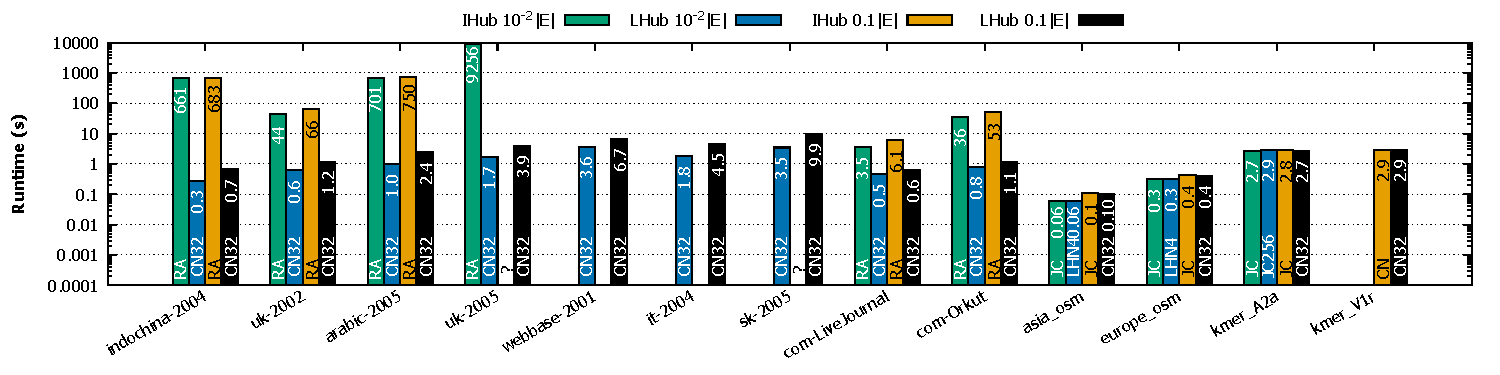
\includegraphics[width=0.98\linewidth]{out/input-large-runtime.pdf}
  }
  \subfigure[Speedup (logarithmic scale) for link prediction with the best similarity measure of \textit{LHub} approach, compared to \textit{IHub} approach]{
    \label{fig:input-large--speedup}
    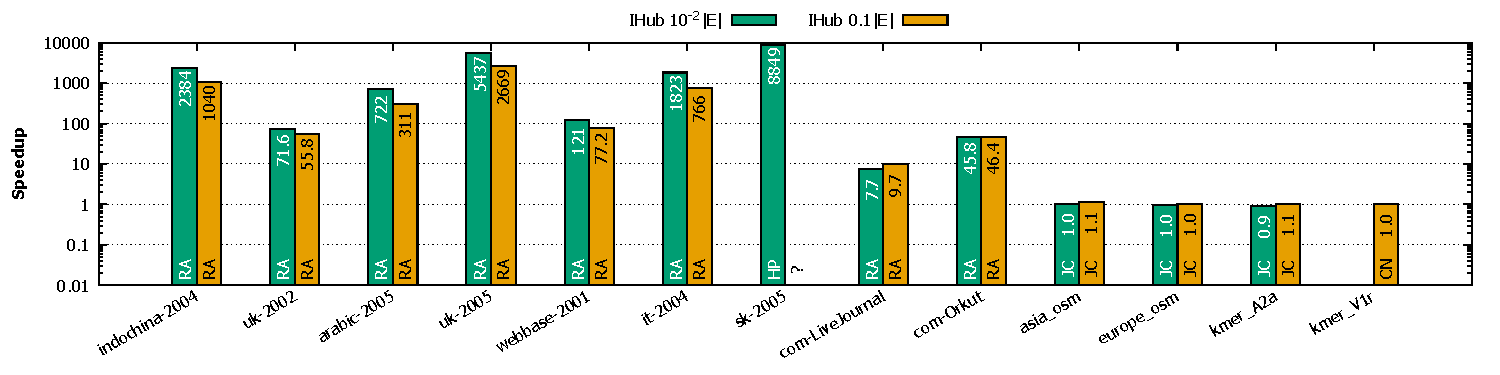
\includegraphics[width=0.98\linewidth]{out/input-large-speedup.pdf}
  }
  \subfigure[F1 score of predicted links (logarithmic scale), for link prediction using the best similarity measure, with \textit{IHub} and \textit{LHub} approaches]{
    \label{fig:input-large--f1score}
    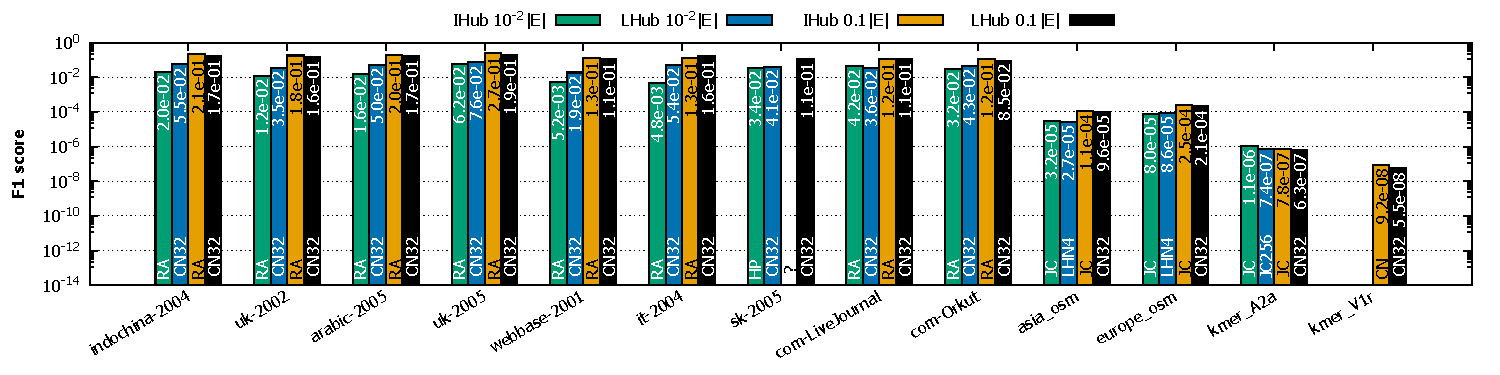
\includegraphics[width=0.98\linewidth]{out/input-large-f1score.pdf}
  } \\[-2ex]
  \caption{Runtime in seconds (log-scale), speedup (log-scale), and F1 score of predicted links (log-scale), for link prediction method using the best similarity measure, when attempting to predict $10^{-2}|E|$ to $0.1|E|$ unobserved edges $E^U$, for each graph in the dataset. For each similarity measure outlined in Section \ref{sec:metrics}, we attempt only the best hub limit $L_H$ parameter setting obtained in Section \ref{sec:select-limit} (for the \textit{LHub} approach), and then select the best among them, considering both the F1 score and runtime. Note that the numerical suffix added to the acronym of each link prediction method, with the \textit{LHub} approach, indicates the hub limit $L_H$ parameter setting.}
  \label{fig:input-large}
\end{figure*}

\begin{figure}[hbtp]
  \centering
  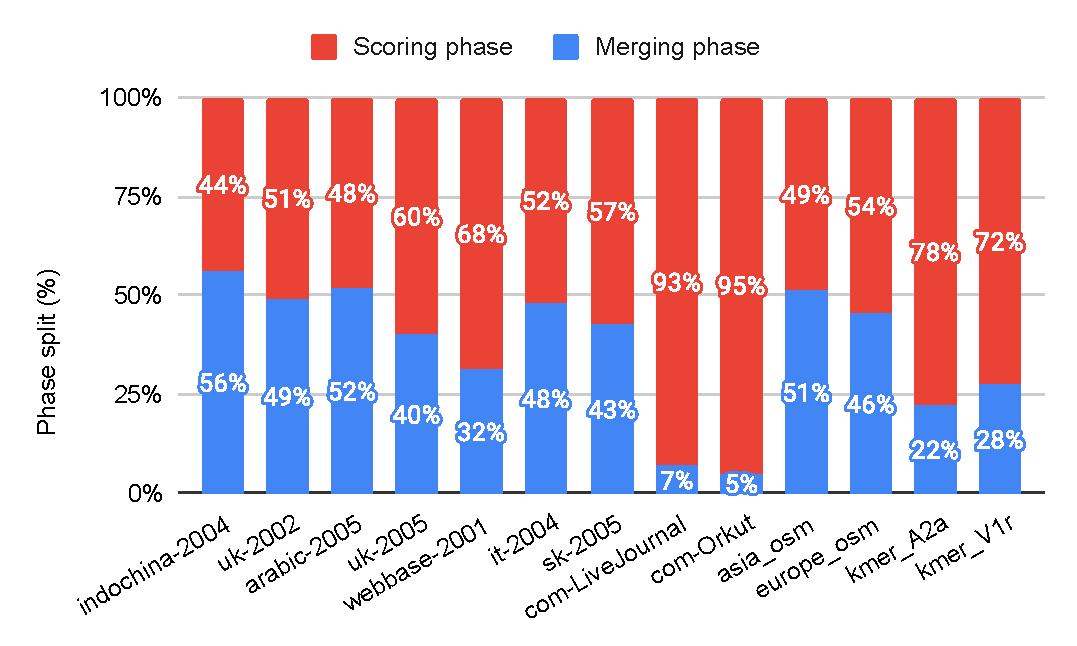
\includegraphics[width=0.98\linewidth]{out/phase-split.pdf} \\[-2ex]
  \caption{Overall phase split of the \textit{LHub} approach, when predicting $0.1|E|$ links with similarity measures given in Section \ref{sec:metrics}, while choosing suitable hub limit $L_H$ setting for each similarity measure as given in Section \ref{sec:select-limit}.}
  \label{fig:phase-split}
\end{figure}

\begin{figure}[hbtp]
  \centering
  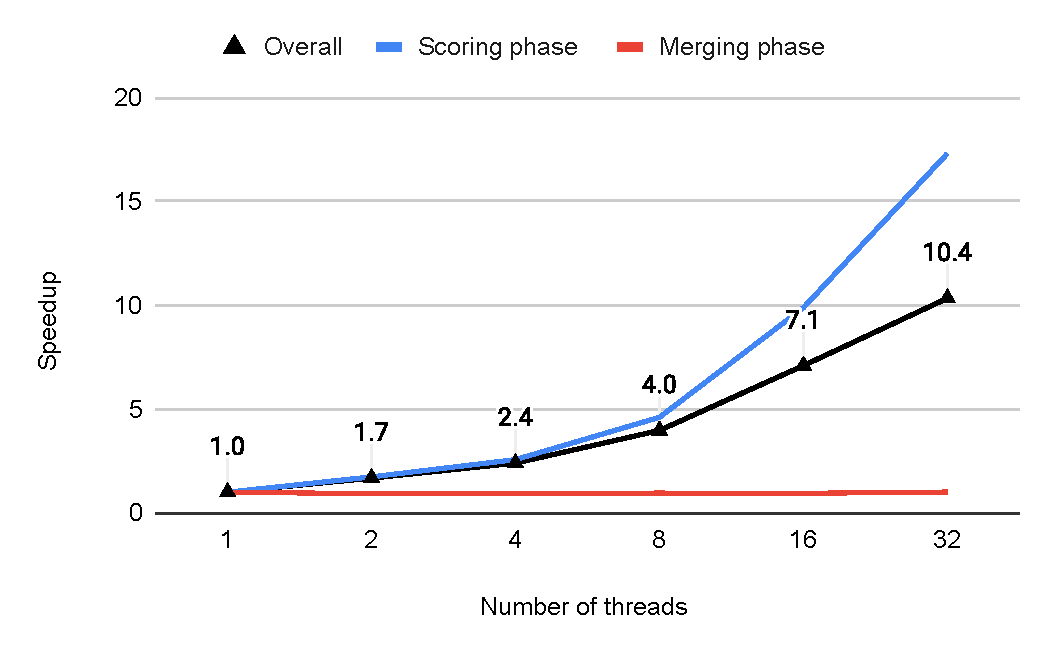
\includegraphics[width=0.98\linewidth]{out/strong-scaling-speedup.pdf} \\[-2ex]
  \caption{Overall speedup of our approach of \textit{Disregarding Large Hubs (DLH)} for link prediction, and its phases (obtaining edges with top-k scores per thread, and merging scores from each thread into a common scoreboard), with $10^{-2}|E|$ unobserved edges, with increasing number of threads (in multiples of 2). Increasing the number of threads causes work in the merging phase to increase,\ignore{thus} leading to a poor speedup.}
  \label{fig:strong-scaling}
\end{figure}


As seen in Figure \ref{fig:input-large}, the DLH approach is, on average, over $1622\times$ and $415\times$ faster than the IBase approach with $10^{-2}|E|$ and $0.1|E|$ unobserved edges, respectively. It achieves this speedup while predicting links with an average F1 score that is $80\%$ higher and $13\%$ lower, respectively --- meaning similar F1 scores without being too low or high. Notably, on the \textit{sk-2005} graph with $0.1|E|$ edges removed, DLH achieves a link prediction rate of $38.1M$ edges/s.

Furthermore, we observe that link prediction with the RA metric excels, in terms of both F1 score and runtime, on web graphs and social networks when using the IBase approach. Meanwhile, link prediction with the JC similarity metric outperforms others on road networks and protein k-mer graphs. With the DLH approach and $10^{-2}|E|$ unobserved edges, link prediction with the CN metric (hub limit $L_H$ of $32$) excels on web graphs and social networks. For road networks, link prediction with the LHN metric (hub limit $L_H$ of $4$) performs the best, and for protein k-mer graphs, link prediction with the JC metric (hub limit $L_H$ of $256$) is optimal. However, with $0.1|E|$ unobserved edges, link prediction with the CN metric (hub limit $L_H$ of $32$) proves to be the best across all graphs. Figures \ref{fig:standard2}, \ref{fig:standard1}, \ref{fig:pruned2}, \ref{fig:pruned1} show the runtimes and F1 scores for link prediction with all similarity measures. Notably, in Figures \ref{fig:pruned2} and \ref{fig:pruned1}, the DLH approach using the AA and RA metrics performs similarly to the CN metric, but with longer runtimes.

Next, we note that the IBase approach achieves an average F1 score of $1.8\times10^{-2}$ and $1.1\times10^{-1}$ when predicting $10^{-2}|E|$ and $0.1|E|$ edges, respectively. In comparison, the DLH approach achieves F1 scores, averaging $3.2\times10^{-2}$ and $9.8\times10^{-2}$, respectively. Additionally, we observe that the F1 score tends to be higher on web graphs and social networks but significantly lower on road networks and protein k-mer graphs. This discrepancy is likely due to the average degree of the graphs, as local/neighborhood-based link prediction methods rely on the neighborhood of vertices up to a distance of $2$. Graphs with lower average degrees provide less information to such methods for predicting edges. While these F1 scores may seem low (compared to the highest possible F1 score of $1$), it's important to consider that they are significantly higher than random predictions. Although machine learning-based approaches might achieve higher F1 scores, neighborhood-based similarity measures excel in computational efficiency (both in terms of runtime and space) and interpretability, as mentioned earlier.

\ignore{Why the choice of best method appears to change with batch size?}
\ignore{Why do these methods perform well?}
\ignore{What we observe on our dataset? What we observe on smaller graphs?}




\subsection{Performance Analysis}

In this section, we examine the phase split of the DLH approach to identify further optimization opportunities. To do this, we generate an observed graph $E^O$ with $0.1|E|$ unobserved edges $E^U$ for each dataset graph using random division, as detailed in Section \ref{sec:generate-batch}. For each observed graph, we predict $0.1|E|$ links using the DLH approach and the similarity measures outlined in Section \ref{sec:metrics}, utilizing the appropriate hub limit $L_H$ value, as per Section \ref{sec:select-limit}.

Figure \ref{fig:phase-split} shows that DLH, spends a majority of its runtime, $63\%$ on average, in the scoring phase. This is particularly notable in social networks with a high average degree. However, a substantial amount of time is still spent on the merging phase, which involves combining predicted edges with top-$k$ scores from each thread into a global top-$k$ list of predicted edges. The sequential nature of the merging phase likely contributes to this runtime, and addressing this aspect is a potential focus for future work.




\subsection{Strong Scaling}

In the final analysis, we evaluate the strong scaling performance of our DLH approach, where we perform link prediction while disregarding large hubs, i.e., first order neighbors with high degree. The assessment involves varying the number of threads from $1$ to $32$ in multiples of $2$ for each input graph. We measure the average time taken to predict $0.1|E|$ links using similarity measures defined in Section \ref{sec:metrics}, incorporating the best hub limit $L_H$ setting identified in Section \ref{sec:select-limit}. Figure \ref{fig:strong-scaling} presents the results, illustrating not only the overall scaling performance but also the scaling of the two phases of each link prediction method: identifying edges with top-$k$ scores in each thread (\textit{scoring phase}) and combining scores across threads to obtain the global top-$k$ edges (\textit{merging phase}).

With $32$ threads, the DLH approach achieves an overall speedup of $10.4\times$ compared to sequential execution, indicating a performance increase of $1.6\times$ for every doubling of threads. The scalability is limited, as the cost of the merging phase increases with an increase in the number of threads, and because the merging is performed with sequential execution. In fact, at $32$ threads, the merging phase obtains no speedup of $1.0\times$, while the scoring phase achieves a speedup of $17.3\times$.
